\documentclass{standalone}
\usepackage{tikz}
\usetikzlibrary{patterns, positioning}


\begin{document}
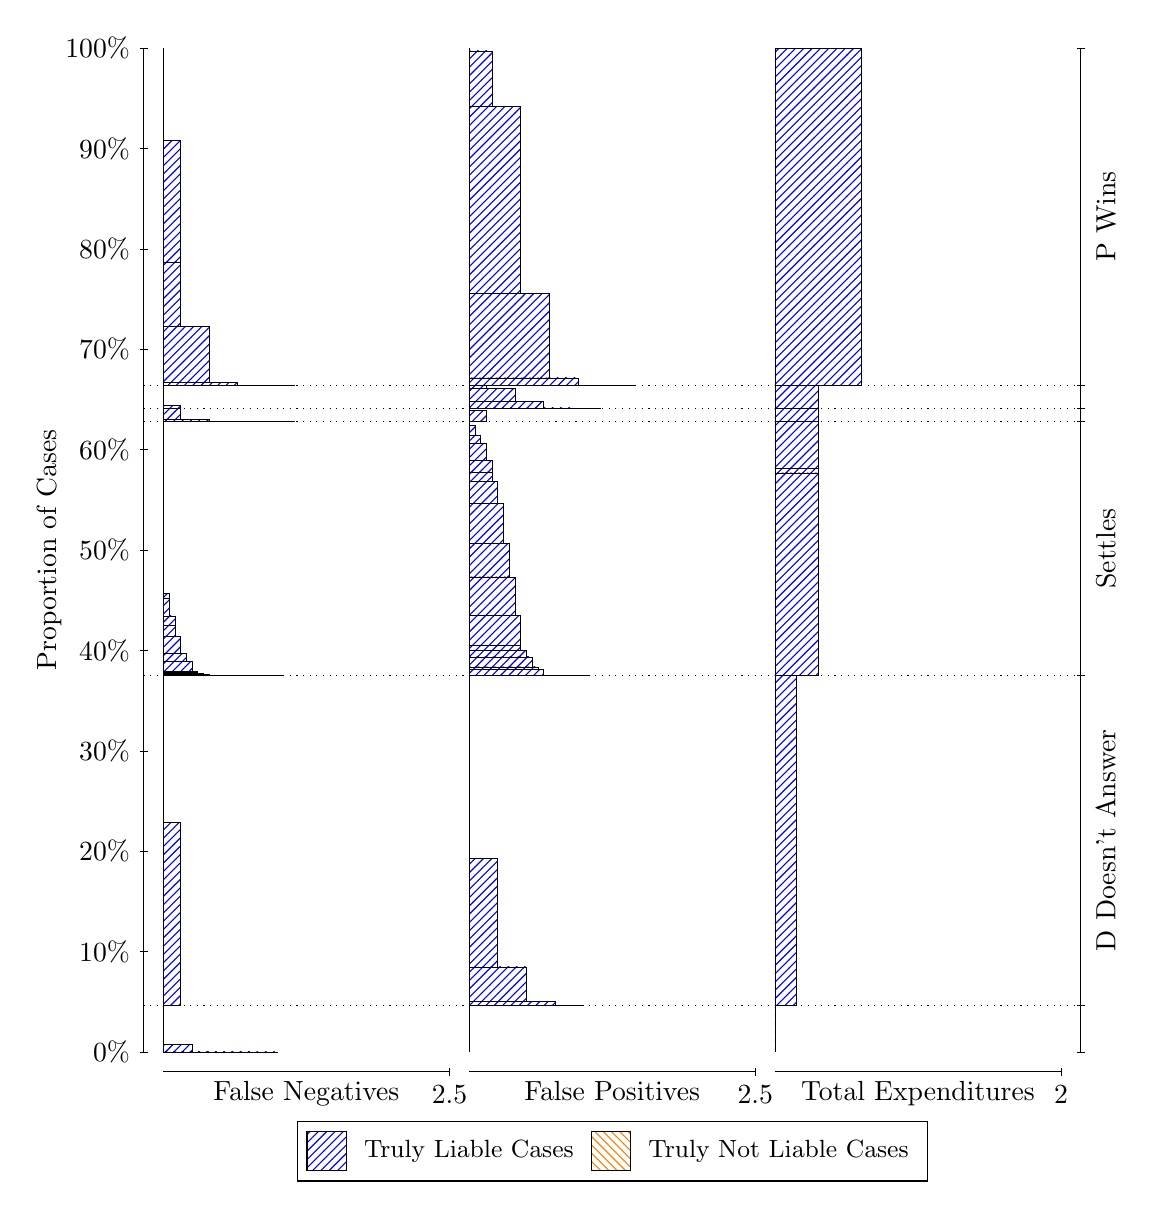
\begin{tikzpicture}
\draw[black, very thin] (1.5,1.75) -- (1.5,14.5);
\node[rotate=90, text=black, anchor=center] at (0.3, 8.125) {Proportion of Cases};
\draw[black, very thin] (1.45,1.75) -- (1.55,1.75);
\node[text=black, anchor=east] at (1.45, 1.75) {0\%};
\draw[black, very thin] (1.45,3.025) -- (1.55,3.025);
\node[text=black, anchor=east] at (1.45, 3.025) {10\%};
\draw[black, very thin] (1.45,4.3) -- (1.55,4.3);
\node[text=black, anchor=east] at (1.45, 4.3) {20\%};
\draw[black, very thin] (1.45,5.575) -- (1.55,5.575);
\node[text=black, anchor=east] at (1.45, 5.575) {30\%};
\draw[black, very thin] (1.45,6.85) -- (1.55,6.85);
\node[text=black, anchor=east] at (1.45, 6.85) {40\%};
\draw[black, very thin] (1.45,8.125) -- (1.55,8.125);
\node[text=black, anchor=east] at (1.45, 8.125) {50\%};
\draw[black, very thin] (1.45,9.4) -- (1.55,9.4);
\node[text=black, anchor=east] at (1.45, 9.4) {60\%};
\draw[black, very thin] (1.45,10.675) -- (1.55,10.675);
\node[text=black, anchor=east] at (1.45, 10.675) {70\%};
\draw[black, very thin] (1.45,11.95) -- (1.55,11.95);
\node[text=black, anchor=east] at (1.45, 11.95) {80\%};
\draw[black, very thin] (1.45,13.225) -- (1.55,13.225);
\node[text=black, anchor=east] at (1.45, 13.225) {90\%};
\draw[black, very thin] (1.45,14.5) -- (1.55,14.5);
\node[text=black, anchor=east] at (1.45, 14.5) {100\%};

\draw[black, very thin] (13.4,1.75) -- (13.4,14.5);
\draw[black, very thin] (13.35,1.75) -- (13.45,1.75);
\node[anchor=west] at (13.35, 1.75) {};
\draw[black, very thin] (13.35,2.3453) -- (13.45,2.3453);
\node[anchor=west] at (13.35, 2.3453) {};
\draw[black, very thin] (13.35,6.5316) -- (13.45,6.5316);
\node[anchor=west] at (13.35, 6.5316) {};
\draw[black, very thin] (13.35,9.7586) -- (13.45,9.7586);
\node[anchor=west] at (13.35, 9.7586) {};
\draw[black, very thin] (13.35,9.9213) -- (13.45,9.9213);
\node[anchor=west] at (13.35, 9.9213) {};
\draw[black, very thin] (13.35,10.215) -- (13.45,10.215);
\node[anchor=west] at (13.35, 10.215) {};
\draw[black, very thin] (13.35,14.5) -- (13.45,14.5);
\node[anchor=west] at (13.35, 14.5) {};

\draw[black, very thin, pattern color=blue, pattern=north east lines] (1.75,1.75) rectangle (3.2033,1.75);
\draw[black, very thin, pattern color=blue, pattern=north east lines] (1.75,1.75) rectangle (2.84,1.75);
\draw[black, very thin, pattern color=blue, pattern=north east lines] (1.75,1.75) rectangle (2.4767,1.7508);
\draw[black, very thin, pattern color=blue, pattern=north east lines] (1.75,1.7508) rectangle (2.1133,1.8475);
\draw[black, very thin, pattern color=orange, pattern=north west lines] (1.75,1.8475) rectangle (1.75,1.8475);
\draw[black, very thin, pattern color=blue, pattern=north east lines] (1.75,1.8475) rectangle (1.75,2.3453);
\draw[black, very thin, pattern color=blue, pattern=north east lines] (1.75,2.3453) rectangle (1.968,4.6683);
\draw[black, very thin, pattern color=orange, pattern=north west lines] (1.75,4.6683) rectangle (1.75,4.6683);
\draw[black, very thin, pattern color=blue, pattern=north east lines] (1.75,4.6683) rectangle (1.75,6.5316);
\draw[black, very thin, pattern color=blue, pattern=north east lines] (1.75,6.5316) rectangle (3.276,6.5316);
\draw[black, very thin, pattern color=blue, pattern=north east lines] (1.75,6.5316) rectangle (3.1307,6.5316);
\draw[black, very thin, pattern color=blue, pattern=north east lines] (1.75,6.5316) rectangle (2.9853,6.5316);
\draw[black, very thin, pattern color=blue, pattern=north east lines] (1.75,6.5316) rectangle (2.9127,6.5316);
\draw[black, very thin, pattern color=blue, pattern=north east lines] (1.75,6.5316) rectangle (2.84,6.5316);
\draw[black, very thin, pattern color=blue, pattern=north east lines] (1.75,6.5316) rectangle (2.7673,6.5316);
\draw[black, very thin, pattern color=blue, pattern=north east lines] (1.75,6.5316) rectangle (2.6947,6.5316);
\draw[black, very thin, pattern color=blue, pattern=north east lines] (1.75,6.5316) rectangle (2.622,6.5317);
\draw[black, very thin, pattern color=blue, pattern=north east lines] (1.75,6.5317) rectangle (2.5493,6.5317);
\draw[black, very thin, pattern color=blue, pattern=north east lines] (1.75,6.5317) rectangle (2.4767,6.5318);
\draw[black, very thin, pattern color=blue, pattern=north east lines] (1.75,6.5318) rectangle (2.404,6.5335);
\draw[black, very thin, pattern color=blue, pattern=north east lines] (1.75,6.5335) rectangle (2.404,6.5335);
\draw[black, very thin, pattern color=blue, pattern=north east lines] (1.75,6.5335) rectangle (2.3313,6.5427);
\draw[black, very thin, pattern color=blue, pattern=north east lines] (1.75,6.5427) rectangle (2.2587,6.5604);
\draw[black, very thin, pattern color=blue, pattern=north east lines] (1.75,6.5604) rectangle (2.186,6.5732);
\draw[black, very thin, pattern color=blue, pattern=north east lines] (1.75,6.5732) rectangle (2.186,6.579);
\draw[black, very thin, pattern color=blue, pattern=north east lines] (1.75,6.579) rectangle (2.1133,6.7107);
\draw[black, very thin, pattern color=blue, pattern=north east lines] (1.75,6.7107) rectangle (2.0407,6.8088);
\draw[black, very thin, pattern color=blue, pattern=north east lines] (1.75,6.8088) rectangle (2.0407,6.8141);
\draw[black, very thin, pattern color=blue, pattern=north east lines] (1.75,6.8141) rectangle (1.968,7.0261);
\draw[black, very thin, pattern color=blue, pattern=north east lines] (1.75,7.0261) rectangle (1.8953,7.172);
\draw[black, very thin, pattern color=blue, pattern=north east lines] (1.75,7.172) rectangle (1.8953,7.2896);
\draw[black, very thin, pattern color=blue, pattern=north east lines] (1.75,7.2896) rectangle (1.8227,7.5158);
\draw[black, very thin, pattern color=blue, pattern=north east lines] (1.75,7.5158) rectangle (1.8227,7.5703);
\draw[black, very thin, pattern color=blue, pattern=north east lines] (1.75,7.5703) rectangle (1.75,7.5718);
\draw[black, very thin, pattern color=orange, pattern=north west lines] (1.75,7.5718) rectangle (1.75,7.5718);
\draw[black, very thin, pattern color=blue, pattern=north east lines] (1.75,7.5718) rectangle (1.75,9.7586);
\draw[black, very thin, pattern color=blue, pattern=north east lines] (1.75,9.7586) rectangle (3.4213,9.7586);
\draw[black, very thin, pattern color=blue, pattern=north east lines] (1.75,9.7586) rectangle (3.058,9.7586);
\draw[black, very thin, pattern color=blue, pattern=north east lines] (1.75,9.7586) rectangle (2.6947,9.7587);
\draw[black, very thin, pattern color=blue, pattern=north east lines] (1.75,9.7587) rectangle (2.3313,9.7801);
\draw[black, very thin, pattern color=blue, pattern=north east lines] (1.75,9.7801) rectangle (1.968,9.9213);
\draw[black, very thin, pattern color=orange, pattern=north west lines] (1.75,9.9213) rectangle (1.75,9.9213);
\draw[black, very thin, pattern color=blue, pattern=north east lines] (1.75,9.9213) rectangle (1.968,9.9633);
\draw[black, very thin, pattern color=orange, pattern=north west lines] (1.75,9.9633) rectangle (1.75,9.9633);
\draw[black, very thin, pattern color=blue, pattern=north east lines] (1.75,9.9633) rectangle (1.75,10.215);
\draw[black, very thin, pattern color=blue, pattern=north east lines] (1.75,10.215) rectangle (3.4213,10.215);
\draw[black, very thin, pattern color=blue, pattern=north east lines] (1.75,10.215) rectangle (3.058,10.215);
\draw[black, very thin, pattern color=blue, pattern=north east lines] (1.75,10.215) rectangle (2.6947,10.253);
\draw[black, very thin, pattern color=blue, pattern=north east lines] (1.75,10.253) rectangle (2.3313,10.961);
\draw[black, very thin, pattern color=blue, pattern=north east lines] (1.75,10.961) rectangle (1.968,11.785);
\draw[black, very thin, pattern color=blue, pattern=north east lines] (1.75,11.785) rectangle (1.968,13.328);
\draw[black, very thin, pattern color=orange, pattern=north west lines] (1.75,13.328) rectangle (1.75,13.328);
\draw[black, very thin, pattern color=blue, pattern=north east lines] (1.75,13.328) rectangle (1.75,14.5);
\draw[black, very thin, pattern color=orange, pattern=north west lines] (5.6333,1.75) rectangle (5.6333,1.75);
\draw[black, very thin, pattern color=blue, pattern=north east lines] (5.6333,1.75) rectangle (5.6333,2.3453);
\draw[black, very thin, pattern color=orange, pattern=north west lines] (5.6333,2.3453) rectangle (7.0867,2.3453);
\draw[black, very thin, pattern color=blue, pattern=north east lines] (5.6333,2.3453) rectangle (7.0867,2.3457);
\draw[black, very thin, pattern color=blue, pattern=north east lines] (5.6333,2.3457) rectangle (6.7233,2.3958);
\draw[black, very thin, pattern color=blue, pattern=north east lines] (5.6333,2.3958) rectangle (6.36,2.83);
\draw[black, very thin, pattern color=blue, pattern=north east lines] (5.6333,2.83) rectangle (5.9967,4.2086);
\draw[black, very thin, pattern color=blue, pattern=north east lines] (5.6333,4.2086) rectangle (5.6333,6.5316);
\draw[black, very thin, pattern color=orange, pattern=north west lines] (5.6333,6.5316) rectangle (7.1593,6.5316);
\draw[black, very thin, pattern color=blue, pattern=north east lines] (5.6333,6.5316) rectangle (7.1593,6.5316);
\draw[black, very thin, pattern color=orange, pattern=north west lines] (5.6333,6.5316) rectangle (7.014,6.5316);
\draw[black, very thin, pattern color=blue, pattern=north east lines] (5.6333,6.5316) rectangle (7.014,6.5316);
\draw[black, very thin, pattern color=orange, pattern=north west lines] (5.6333,6.5316) rectangle (6.8687,6.5316);
\draw[black, very thin, pattern color=blue, pattern=north east lines] (5.6333,6.5316) rectangle (6.8687,6.5318);
\draw[black, very thin, pattern color=blue, pattern=north east lines] (5.6333,6.5318) rectangle (6.796,6.5335);
\draw[black, very thin, pattern color=orange, pattern=north west lines] (5.6333,6.5335) rectangle (6.7233,6.5335);
\draw[black, very thin, pattern color=blue, pattern=north east lines] (5.6333,6.5335) rectangle (6.7233,6.534);
\draw[black, very thin, pattern color=blue, pattern=north east lines] (5.6333,6.534) rectangle (6.6507,6.5363);
\draw[black, very thin, pattern color=orange, pattern=north west lines] (5.6333,6.5363) rectangle (6.578,6.5363);
\draw[black, very thin, pattern color=blue, pattern=north east lines] (5.6333,6.5363) rectangle (6.578,6.6048);
\draw[black, very thin, pattern color=blue, pattern=north east lines] (5.6333,6.6048) rectangle (6.5053,6.6406);
\draw[black, very thin, pattern color=orange, pattern=north west lines] (5.6333,6.6406) rectangle (6.4327,6.6406);
\draw[black, very thin, pattern color=blue, pattern=north east lines] (5.6333,6.6406) rectangle (6.4327,6.7679);
\draw[black, very thin, pattern color=orange, pattern=north west lines] (5.6333,6.7679) rectangle (6.4327,6.7679);
\draw[black, very thin, pattern color=blue, pattern=north east lines] (5.6333,6.7679) rectangle (6.4327,6.768);
\draw[black, very thin, pattern color=blue, pattern=north east lines] (5.6333,6.768) rectangle (6.36,6.8515);
\draw[black, very thin, pattern color=blue, pattern=north east lines] (5.6333,6.8515) rectangle (6.2873,6.9152);
\draw[black, very thin, pattern color=orange, pattern=north west lines] (5.6333,6.9152) rectangle (6.2873,6.9152);
\draw[black, very thin, pattern color=blue, pattern=north east lines] (5.6333,6.9152) rectangle (6.2873,7.2995);
\draw[black, very thin, pattern color=blue, pattern=north east lines] (5.6333,7.2995) rectangle (6.2147,7.7836);
\draw[black, very thin, pattern color=orange, pattern=north west lines] (5.6333,7.7836) rectangle (6.142,7.7836);
\draw[black, very thin, pattern color=blue, pattern=north east lines] (5.6333,7.7836) rectangle (6.142,8.2105);
\draw[black, very thin, pattern color=blue, pattern=north east lines] (5.6333,8.2105) rectangle (6.0693,8.7184);
\draw[black, very thin, pattern color=blue, pattern=north east lines] (5.6333,8.7184) rectangle (6.0693,8.7199);
\draw[black, very thin, pattern color=orange, pattern=north west lines] (5.6333,8.7199) rectangle (5.9967,8.7199);
\draw[black, very thin, pattern color=blue, pattern=north east lines] (5.6333,8.7199) rectangle (5.9967,9.0006);
\draw[black, very thin, pattern color=blue, pattern=north east lines] (5.6333,9.0006) rectangle (5.924,9.1183);
\draw[black, very thin, pattern color=blue, pattern=north east lines] (5.6333,9.1183) rectangle (5.924,9.2641);
\draw[black, very thin, pattern color=blue, pattern=north east lines] (5.6333,9.2641) rectangle (5.8513,9.4761);
\draw[black, very thin, pattern color=blue, pattern=north east lines] (5.6333,9.4761) rectangle (5.7787,9.5795);
\draw[black, very thin, pattern color=blue, pattern=north east lines] (5.6333,9.5795) rectangle (5.706,9.7111);
\draw[black, very thin, pattern color=blue, pattern=north east lines] (5.6333,9.7111) rectangle (5.706,9.7112);
\draw[black, very thin, pattern color=blue, pattern=north east lines] (5.6333,9.7112) rectangle (5.6333,9.7586);
\draw[black, very thin, pattern color=orange, pattern=north west lines] (5.6333,9.7586) rectangle (5.8513,9.7586);
\draw[black, very thin, pattern color=blue, pattern=north east lines] (5.6333,9.7586) rectangle (5.8513,9.8998);
\draw[black, very thin, pattern color=blue, pattern=north east lines] (5.6333,9.8998) rectangle (5.6333,9.9213);
\draw[black, very thin, pattern color=orange, pattern=north west lines] (5.6333,9.9213) rectangle (7.3047,9.9213);
\draw[black, very thin, pattern color=blue, pattern=north east lines] (5.6333,9.9213) rectangle (7.3047,9.9214);
\draw[black, very thin, pattern color=blue, pattern=north east lines] (5.6333,9.9214) rectangle (6.9413,9.9312);
\draw[black, very thin, pattern color=blue, pattern=north east lines] (5.6333,9.9312) rectangle (6.578,10.016);
\draw[black, very thin, pattern color=blue, pattern=north east lines] (5.6333,10.016) rectangle (6.2147,10.173);
\draw[black, very thin, pattern color=blue, pattern=north east lines] (5.6333,10.173) rectangle (5.8513,10.215);
\draw[black, very thin, pattern color=orange, pattern=north west lines] (5.6333,10.215) rectangle (7.7407,10.215);
\draw[black, very thin, pattern color=blue, pattern=north east lines] (5.6333,10.215) rectangle (7.7407,10.215);
\draw[black, very thin, pattern color=orange, pattern=north west lines] (5.6333,10.215) rectangle (7.3773,10.215);
\draw[black, very thin, pattern color=blue, pattern=north east lines] (5.6333,10.215) rectangle (7.3773,10.217);
\draw[black, very thin, pattern color=orange, pattern=north west lines] (5.6333,10.217) rectangle (7.014,10.217);
\draw[black, very thin, pattern color=blue, pattern=north east lines] (5.6333,10.217) rectangle (7.014,10.31);
\draw[black, very thin, pattern color=orange, pattern=north west lines] (5.6333,10.31) rectangle (6.6507,10.31);
\draw[black, very thin, pattern color=blue, pattern=north east lines] (5.6333,10.31) rectangle (6.6507,11.387);
\draw[black, very thin, pattern color=orange, pattern=north west lines] (5.6333,11.387) rectangle (6.2873,11.387);
\draw[black, very thin, pattern color=blue, pattern=north east lines] (5.6333,11.387) rectangle (6.2873,13.754);
\draw[black, very thin, pattern color=blue, pattern=north east lines] (5.6333,13.754) rectangle (5.924,14.463);
\draw[black, very thin, pattern color=blue, pattern=north east lines] (5.6333,14.463) rectangle (5.6333,14.5);
\draw[black, very thin, pattern color=orange, pattern=north west lines] (9.5167,1.75) rectangle (9.5167,1.75);
\draw[black, very thin, pattern color=blue, pattern=north east lines] (9.5167,1.75) rectangle (9.5167,2.3453);
\draw[black, very thin, pattern color=orange, pattern=north west lines] (9.5167,2.3453) rectangle (9.7892,2.3453);
\draw[black, very thin, pattern color=blue, pattern=north east lines] (9.5167,2.3453) rectangle (9.7892,6.5316);
\draw[black, very thin, pattern color=orange, pattern=north west lines] (9.5167,6.5316) rectangle (10.062,6.5316);
\draw[black, very thin, pattern color=blue, pattern=north east lines] (9.5167,6.5316) rectangle (10.062,9.1037);
\draw[black, very thin, pattern color=orange, pattern=north west lines] (9.5167,9.1037) rectangle (10.062,9.1037);
\draw[black, very thin, pattern color=blue, pattern=north east lines] (9.5167,9.1037) rectangle (10.062,9.164);
\draw[black, very thin, pattern color=orange, pattern=north west lines] (9.5167,9.164) rectangle (10.062,9.164);
\draw[black, very thin, pattern color=blue, pattern=north east lines] (9.5167,9.164) rectangle (10.062,9.7586);
\draw[black, very thin, pattern color=orange, pattern=north west lines] (9.5167,9.7586) rectangle (10.062,9.7586);
\draw[black, very thin, pattern color=blue, pattern=north east lines] (9.5167,9.7586) rectangle (10.062,9.9213);
\draw[black, very thin, pattern color=orange, pattern=north west lines] (9.5167,9.9213) rectangle (10.062,9.9213);
\draw[black, very thin, pattern color=blue, pattern=north east lines] (9.5167,9.9213) rectangle (10.062,10.215);
\draw[black, very thin, pattern color=orange, pattern=north west lines] (9.5167,10.215) rectangle (10.607,10.215);
\draw[black, very thin, pattern color=blue, pattern=north east lines] (9.5167,10.215) rectangle (10.607,14.5);
\draw[black, dotted] (1.5,2.3453) -- (13.4,2.3453);
\draw[black, dotted] (1.5,6.5316) -- (13.4,6.5316);
\draw[black, dotted] (1.5,9.7586) -- (13.4,9.7586);
\draw[black, dotted] (1.5,9.9213) -- (13.4,9.9213);
\draw[black, dotted] (1.5,10.215) -- (13.4,10.215);
\draw[black, very thin] (1.75,1.5) -- (5.3833,1.5);
\node[text=black, anchor=north] at (3.5667, 1.5) {False Negatives};
\draw[black, very thin] (5.3833,1.45) -- (5.3833,1.55);
\node[text=black, anchor=north] at (5.3833, 1.45) {2.5};

\draw[black, very thin] (5.6333,1.5) -- (9.2667,1.5);
\node[text=black, anchor=north] at (7.45, 1.5) {False Positives};
\draw[black, very thin] (9.2667,1.45) -- (9.2667,1.55);
\node[text=black, anchor=north] at (9.2667, 1.45) {2.5};

\draw[black, very thin] (9.5167,1.5) -- (13.15,1.5);
\node[text=black, anchor=north] at (11.333, 1.5) {Total Expenditures};
\draw[black, very thin] (13.15,1.45) -- (13.15,1.55);
\node[text=black, anchor=north] at (13.15, 1.45) {2};


\node[text=black, centered, rotate=90] at (13.72, 4.4385) {D Doesn't Answer};
\node[text=black, centered, rotate=90] at (13.72, 8.1451) {Settles};


\node[text=black, centered, rotate=90] at (13.72, 12.358) {P Wins};

\draw (7.449999999999999,1.5) node[draw=none] (baseCoordinate) {};
\begin{scope}[align=center]
        \matrix[scale=0.5, draw=black, below=0.5cm of baseCoordinate, nodes={draw}, column sep=0.1cm]{
            \node[rectangle, draw, minimum width=0.5cm, minimum height=0.5cm, pattern color=blue, pattern=north east lines] {}; &
            \node[draw=none, font=\small, text=black] (B) {Truly Liable Cases}; &
            \node[rectangle, draw, minimum width=0.5cm, minimum height=0.5cm, pattern color=orange, pattern=north west lines] {}; &
            \node[draw=none, font=\small, text=black] (B) {Truly Not Liable Cases}; \\
            };
\end{scope}

\end{tikzpicture}
\end{document}